\begin{figure}[h!]
    \centering
    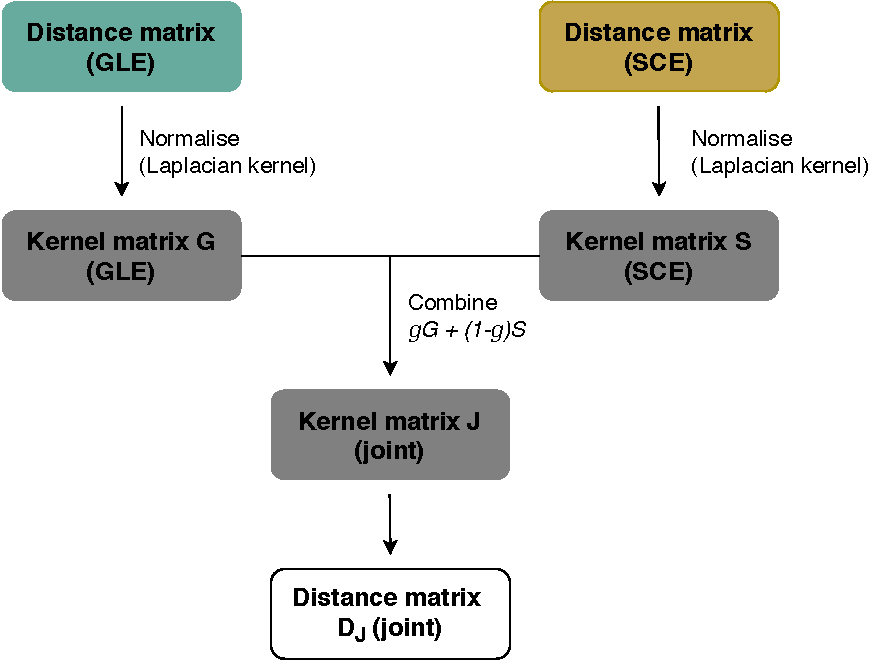
\includegraphics[scale=0.8]{graphics/joint_classifier.pdf}
\caption{}
    % \caption{\textbf{Summary of the methods to train the joint classifier for GLE and SCE}. The pairwise distance matrix for each factor was converted to a kernel matrix, normalised and linearly combined with weights $g$ and $1-g$ to get the joint kernel matrix $J$ (equation \ref{eq:joint}). $J$ was then converted back to a distance matrix $D_J$ using equation \ref{eq:k2d}. $D_J$ was subsequently used for model training.}
    \label{fig:joint}
\end{figure}
